\documentclass[]{scrartcl}

%opening
\title{Rotating magneto-hydrodynamics}
\author{J. Lara \& S. Glane}

\usepackage{amsmath}
\usepackage{amssymb}
\usepackage{amsfonts}
\usepackage{mathtools}
\usepackage{xfrac}
\usepackage{siunitx}
\usepackage{hyperref}
\usepackage{cleveref}
\newcommand{\pfrac}[2]{\frac{\partial #1}{\partial #2}}
\newcommand{\tdfrac}[2]{\frac{\mathrm{d} #1}{\mathrm{d} #2}}
\renewcommand{\d}{\,\mathrm{d}}
\newcommand{\bs}[1]{\boldsymbol{#1}}
\newcommand{\abs}[1]{\left\lvert #1 \right\rvert}
\newcommand{\norm}[1]{\left\lVert #1 \right\rVert}
\DeclareMathOperator{\divv}{div}
\DeclareMathOperator{\grad}{grad}
\DeclareMathOperator{\rot}{rot}
\DeclareMathOperator{\cof}{Cof}
\DeclareMathOperator{\Spur}{Sp}
\DeclareMathOperator{\Sgn}{sgn}
\DeclareMathOperator{\Sym}{sym}

\newcommand{\alignedintertext}[1]{%
	\noalign{%
		\vskip\belowdisplayshortskip
		\vtop{\hsize=\linewidth#1\par
			\expandafter}%
		\expandafter\prevdepth\the\prevdepth
	}%
}

\begin{document}

\maketitle

\begin{abstract}

\end{abstract}

\section{Fluid mechanics}\label{Sec:FluidMechanics}
A \textbf{purely mechanical analysis} of a fluid reduces to the momentum and mass conservation. Their local forms are given
\begin{equation*}
	\begin{aligned}
		\rho \tdfrac{\mathbf{v}}{t} &= \nabla \cdot \mathbf{T} + \rho \mathbf{b}, &\forall (\mathbf{x}, t) \in \Omega \times \left[0, T \right] \\
		\tdfrac{\rho}{t} + \rho \nabla \cdot \mathbf{v}&= 0, &\forall (\mathbf{x}, t) \in \Omega \times  \left[0, T \right]
	\end{aligned}
\end{equation*} 
where $\rho$ is the density, $\mathbf{v}$ the velocity, $\mathbf{T}$ the stress tensor and $\mathbf{f}$ the volumetric forces. Furthermore $\mathbf{x}$ denotes the position vector, $t$ the time, $\Omega$  $n$-dimensional domain $\Omega \subset \mathbb{R}^n$ and $T$ the upper limit of the temporal space. The field equations need to be complemented with initial and boundary conditions and a constitutive equation for the stress in order for them to be solvable. For \textbf{linear viscous and isotropic} fluids the stress tensor is given by
\begin{equation*}
	\mathbf{T} = (-p + \lambda \Spur \mathbf{D}) \mathbf{I} + 2 \mu \mathbf{D}
\end{equation*}
Here $p$ denotes the hydrostatic pressure, $\lambda$ the bulk viscosity, $\mu$ the dynamic viscosity, $\mathbf{D} = \Sym (\nabla \otimes \mathbf{v})$ the symmetric part of the velocity gradient and $\mathbf{I}$ the second order identity tensor. \textbf{Assuming that $\lambda$ and $\mu$ are constants}, the momentum field equation becomes
\begin{equation*}
\rho \tdfrac{\mathbf{v}}{t} = -\nabla p + (\lambda + \mu) \nabla (\nabla \cdot \mathbf{v}) + \mu \Delta \mathbf{v} + \rho\mathbf{b}, \quad \forall (\mathbf{x}, t) \in \Omega \times \left[0, T \right]
\end{equation*}
For the case of an \textbf{incompressible flow}, i.e. $\nabla \cdot \mathbf{v} = 0$, and expanding the material time derivative, the field equations reduce further to
\begin{equation*}
	\begin{aligned}
		\rho \pfrac{\mathbf{v}}{t} +  \rho \mathbf{v} \cdot (\nabla \otimes \mathbf{v})&=  -\nabla p + \mu \Delta \mathbf{v} + \rho \mathbf{b}, &\forall (\mathbf{x}, t) \in \Omega \times \left[0, T \right] \\
		\nabla \cdot \mathbf{v}&= 0, &\forall (\mathbf{x}, t) \in \Omega \times  \left[0, T \right]
	\end{aligned}
\end{equation*}
\textbf{Assuming the density to be constant}, it is customary to divide the momentum equation with it, which leads to 
\begin{equation*}
	\begin{aligned}
		\pfrac{\mathbf{v}}{t} + \mathbf{v} \cdot (\nabla \otimes \mathbf{v})&=  - \dfrac{1}{\rho}\nabla p + \nu \Delta \mathbf{v} + \mathbf{b}, &\forall (\mathbf{x}, t) \in \Omega \times \left[0, T \right] \\
		\nabla \cdot \mathbf{v}&= 0, &\forall (\mathbf{x}, t) \in \Omega \times  \left[0, T \right]
	\end{aligned}
\end{equation*}
where $\nu = \sfrac{\mu}{\rho}$ is the kinematic viscosity. The dimensionless form of this set of field equations is obtained by introducing a multiplicative decomposition of a arbitrary tensor $\bs{\phi}$
\begin{equation*}
	\bs{\phi} = \hat{\phi} \tilde{\bs{\phi}}
\end{equation*}
Here is $\hat{\phi}$ a constant scalar, seen as an scaling factor, and $ \tilde{\bs{\phi}}$ a dimensionless tensor. By implementing the decomposition, the field equations become
\begin{equation*}
	\begin{aligned}
		\pfrac{\mathbf{\tilde{v}}}{\tilde{t}} + \mathbf{\tilde{v}} \cdot (\tilde{\nabla} \otimes \mathbf{\tilde{v}})&=  -\tilde{\nabla} \tilde{p}+ \dfrac{1}{\mathrm{Re}}\tilde{\Delta} \mathbf{\tilde{v}} + \mathbf{\tilde{b}}, &\forall (\mathbf{\tilde{x}}, \tilde{t}) \in \tilde{\Omega} \times [0, \tilde{T} ] \\
		\tilde{\nabla} \cdot \mathbf{\tilde{v}}&= 0, &\forall (\mathbf{\tilde{x}}, \tilde{t}) \in\tilde{ \Omega} \times  [0, \tilde{T} ]
	\end{aligned}
\end{equation*}
where $\mathrm{Re} = \hat{v}L_\textrm{c}\nu^{-1}$ is the \textsc{Reynolds} number. Note that the scaling factor of the position vector is set as a characteristic length of the problem, i.e. $\hat{x} = L_\textrm{c}$. Consistently, the characteristic time is set to $\hat{t} = \sfrac{L_\textrm{c}}{\hat{v}}$. Furthermore, pressure scaling and volumemetric force scaling were set to $\hat{p} = \rho \hat{v}^2$ and $\hat{b} = \hat{v}\hat{t}^{-1}$ respectively. \textbf{From here on now the tildes are going to be obviated, but keep in mind we are working with the dimensionless form of the field equations}.\\

\section{Treatment of the convection term}

\begin{itemize}
	\item skew-symmetric form
	\begin{equation*}
		\mathbf{u} \cdot (\nabla \otimes \mathbf{u}) + \dfrac{1}{2} (\nabla \cdot \mathbf{u})\mathbf{u}
	\end{equation*}
	\item divergence form
	\begin{equation*}
		\mathbf{u} \cdot (\nabla \otimes \mathbf{u}) + (\nabla \cdot \mathbf{u})\mathbf{u}
	\end{equation*}
	\item rotational form
	\begin{equation*}
		(\nabla \times \mathbf{u}) \times \mathbf{u}
	\end{equation*}
\end{itemize}


\section{Projection methods: Pressure-correction schemes}
The momentum equation and mass conservation field equations are meant to be solved simultaneously to find $\mathbf{v}$ and $p$. For large problems this can be cumbersome and, above all, very slow. The projection methods aim to decouple the field equations. In the case of the pressure-correction schemes this is done by introducing a velocity field $\mathbf{u}$, which is not divergence free, and splitting the momentum equation into two equations. This is better explained by looking specific schemes up. But first we formally define the problem
\begin{alignat*}{2}
	\pfrac{\mathbf{v}}{t}  + \mathbf{v}\cdot (\nabla \otimes \mathbf{v}) &=  -\nabla p  +  \mathrm{Re}^{-1} \Delta \mathbf{v} + \mathbf{b}, \quad &\forall (\mathbf{x}, t) &\in \Omega \times \left[0, T \right] \\
	\nabla \cdot \mathbf{v} &= 0, &\forall (\mathbf{x}, t) &\in \Omega \times \left[0, T \right] \\
	\intertext{with boundary conditions,}
	\mathbf{v} &= \mathbf{v}_\textrm{D} &\forall\left(\mathbf{x}, t\right) &\in \Gamma_\textrm{D} \times \left[0, T \right] \\ 
	[-p \mathbf{I} + (\rho\textrm{Re})^{-1}\nabla \otimes \mathbf{v}]\cdot \mathbf{n} &= \mathbf{t}_\textrm{N}, &\forall \left(\mathbf{x}, t\right) &\in \Gamma_\textrm{N} \times \left[0, T \right] \\
	\intertext{and initial condtion,} 
	\mathbf{v} &= \mathbf{v}_0, &\forall (\mathbf{x}, 0) &\in \Omega
\end{alignat*}
where $\mathbf{v}_\textrm{D}$ denotes the velocity at the \textsc{Dirichlet} boundary $\Gamma_\textrm{D}\subset\partial\Omega$, $\mathbf{t}_\textrm{N}$ the traction vector at the \textsc{Neumann} boundary $\Gamma_\textrm{N}\subset\partial\Omega$, $\mathbf{t}_\textrm{N}$, with $\partial \Omega = \Gamma_\textrm{D} \cup \Gamma_\textrm{N}$ and $ \Gamma_\textrm{D} \cap \Gamma_\textrm{N} = \emptyset$, and $\mathbf{v}_0$ is the initial velocity. As a remainder, the stated problem is dimensionless. Therefore the boundary and initial conditions are also in their dimensionless form.
\subsection{Incremental scheme in standard form}
By implementing a BDF2 scheme for the time derivative and adding an auxiliary velocity field $\mathbf{u}$, which is not divergence free but fulfills the \textsc{Dirichlet} boundary conditions, and the pressure from the previous time step to the mix we become
\begin{equation*}
\begin{split}
	\dfrac{0.5}{\Delta t} \left[3\mathbf{v}^{k} + 3\mathbf{u}^{k} - 3\mathbf{u}^{k} - 4\mathbf{v}^{k-1} + \mathbf{v}^{k-2}\right]  + \mathbf{v}^{k} \cdot (\nabla \otimes \mathbf{v}^{k})= \\  -\nabla (p^{k} + p^{k-1} - p^{k+1}) +  \mathrm{Re}^{-1} \Delta \mathbf{v}^{k} + \mathbf{b}^{k}
\end{split}
\end{equation*}
which is now split into
\begin{equation*}
	\begin{aligned}
		\dfrac{0.5}{\Delta t} \left[3\mathbf{u}^{k} - 4\mathbf{v}^{k-1} + \mathbf{v}^{k-2}\right]  + \mathbf{v}^{k} \cdot (\nabla \otimes \mathbf{v}^{k}) &= -\nabla p^{k-1} +  \mathrm{Re}^{-1} \Delta \mathbf{v}^{k} + \mathbf{b}^{k} \\
		\dfrac{0.5}{\Delta t} \left[3\mathbf{v}^{k} - 3\mathbf{u}^{k} \right] &= -\nabla (p^{k} - p^{k-1})
	\end{aligned}
\end{equation*}
The decoupling takes places by replacing $\mathbf{v}^{k}$ by $\mathbf{u}^{k}$ in the convective and diffusive terms and solving the first equation without taking the incompressibilty condition in consideration, i.e.
\begin{equation*}
	\begin{aligned}
		\dfrac{0.5}{\Delta t} \left[3\mathbf{u}^{k} - 4\mathbf{v}^{k-1} + \mathbf{v}^{k-2}\right]  + \mathbf{u}^{k} \cdot (\nabla \otimes \mathbf{u}^{k}) &= -\nabla p^{k-1} +  \mathrm{Re}^{-1} \Delta \mathbf{u}^{k} + \mathbf{b}^{k}, &\forall (\mathbf{x}, t) &\in \Omega \times \left[0, T \right]  \\
		\mathbf{u}^{k} &= \mathbf{v}_\textrm{D}, &\forall (\mathbf{x}, t) &\in \Gamma_\textrm{D} \times \left[0, T \right] \\
		[-p^{k-1} \mathbf{I} + (\rho\textrm{Re})^{-1}\nabla \otimes \mathbf{u}^{k}]\cdot \mathbf{n} &= \mathbf{t}_\textrm{N}, &\forall \left(\mathbf{x}, t\right) &\in \Gamma_\textrm{N} \times \left[0, T \right]
	\end{aligned}
\end{equation*}
which is called the viscous or diffusion step. The second equation is coupled with the incompressibility condition to form the projection step
\begin{equation*}
\begin{aligned}
		\dfrac{0.5}{\Delta t} \left[3\mathbf{v}^{k} - 3\mathbf{u}^{k} \right] &= -\nabla (p^{k} - p^{k-1}), &\forall (\mathbf{x}, t) &\in \Omega \times \left[0, T \right] \\
		\nabla \cdot \mathbf{v}^{k} &= 0, &\forall (\mathbf{x}, t) &\in \Omega \times \left[0, T \right] \\
	\nabla(p^{k} - p^{k-1}) \cdot \mathbf{n} &= 0, &\forall (\mathbf{x}, t) &\in \Gamma_\textrm{D} \times \left[0, T \right] \\
		p^{k} - p^{k-1} &=0, &\forall\left(\mathbf{x}, t\right) &\in \Gamma_\textrm{N} \times \left[0, T \right]
\end{aligned}	
\end{equation*}
By applying the divergence operator to the equation and introducing an auxiliary variable $\phi^{k} = p^{k} - p^{k-1}$ , the whole step can be reduced to
\begin{equation*}
\begin{aligned}
	\Delta \phi^{k} &= \dfrac{1.5}{\Delta t} \nabla \cdot \mathbf{u}^{k},  &\forall (\mathbf{x}, t) &\in \Omega \times \left[0, T \right] \\
	\nabla \phi^{k} \cdot \mathbf{n} &= 0, &\forall (\mathbf{x}, t) &\in \Gamma_\textrm{D} \times \left[0, T \right] \\
	\phi^{k} &= 0, &\forall\left(\mathbf{x}, t\right) &\in \Gamma_\textrm{N} \times \left[0, T \right]
\end{aligned}
\end{equation*}
The first boundary condition is an artificial boundary condition which reduces the order of the scheme in its $L^2$ and $H^1$ norms. The last step of the pressure-correction scheme is called correction or update step. As the name implies the velocity $\mathbf{v}^{k}$ and pressure $p^{k}$ are computed by
\begin{equation*}
\begin{aligned}
	\mathbf{v}^{k} &= \mathbf{u}^{k} - \dfrac{\Delta t}{1.5} \nabla \phi^{k} \\
	p^{k} &= p^{k-1} + \phi^{k}
\end{aligned}
\end{equation*}
\subsection{Incremental scheme in rotational form}
The rotational form implements the same diffusion step
\begin{equation*}
	\begin{aligned}
		\dfrac{0.5}{\Delta t} \left[3\mathbf{u}^{k} - 4\mathbf{v}^{k-1} + \mathbf{v}^{k-2}\right]  + \mathbf{u}^{k} \cdot (\nabla \otimes \mathbf{u}^{k}) &= -\nabla p^{k-1} +  \mathrm{Re}^{-1} \Delta \mathbf{u}^{k} + \mathbf{b}^{k}, &\forall (\mathbf{x}, t) &\in \Omega \times \left[0, T \right]  \\
		\mathbf{u}^{k} &= \mathbf{v}_\textrm{D}, &\forall (\mathbf{x}, t) &\in \Gamma_\textrm{D} \times \left[0, T \right] \\
		[-p^{k-1} \mathbf{I} + (\rho\textrm{Re})^{-1}\nabla \otimes \mathbf{u}^{k}]\cdot \mathbf{n} &= \mathbf{t}_\textrm{N}, &\forall \left(\mathbf{x}, t\right) &\in \Gamma_\textrm{N} \times \left[0, T \right]
	\end{aligned}
\end{equation*}
and the same scheme of projection step
\begin{equation*}
	\begin{aligned}
		\Delta \phi^{k} &= \dfrac{1.5}{\Delta t} \nabla \cdot \mathbf{u}^{k},  &\forall (\mathbf{x}, t) &\in \Omega \times \left[0, T \right] \\
		\nabla \phi^{k} \cdot \mathbf{n} &= 0, &\forall (\mathbf{x}, t) &\in \Gamma_\textrm{D} \times \left[0, T \right] \\
		\phi^{k} &= 0, &\forall\left(\mathbf{x}, t\right) &\in \Gamma_\textrm{N} \times \left[0, T \right]
	\end{aligned}
\end{equation*}
with the exception that the auxiliary variable is defines as
\begin{equation*}
	\phi^{k} = p^{k} - p^{k-1} + \textrm{Re}^{-1} \nabla \cdot \mathbf{u}^{k}
\end{equation*}
The update of the velocity and the pressure is given then by
\begin{equation*}
	\begin{aligned}
		\mathbf{v}^{k} &= \mathbf{u}^{k} - \dfrac{\Delta t}{1.5} \nabla \phi^{k} \\
		p^{k} &= p^{k-1} + \phi^{k} -  \textrm{Re}^{-1} \nabla \cdot \mathbf{u}^{k}
	\end{aligned}
\end{equation*}
 From the first equation of the projection step, before applying the divergence to it, 
\begin{equation*}
\dfrac{0.5}{\Delta t} \left[3\mathbf{v}^{k} - 3\mathbf{u}^{k} \right] = -\nabla \phi^{k}
\end{equation*}
it is easy to see that $\nabla \times \nabla \times \mathbf{u} = \nabla \times \nabla \times \mathbf{v}$. Furthermore by adding the above equation to the diffusion step, using the identity $\nabla \times \nabla \times \mathbf{a} = \nabla (\nabla \cdot \mathbf{a}) - \Delta \mathbf{a}$ and coupling the result again with the incompressibility condition we get the \textsc{Navier-Stokes} equations again. This form greatly improves the deficiencies of the standard form due to boundary layer created by the artifical boundary condition. 

\subsection{Generalized incremental scheme}
The standard and rotational forms can be generalized into one scheme using a backward difference formula of $q$-order (BDF$q$) by defining the time derivative
\begin{equation*}
	\pfrac{\mathbf{v}}{t} = \dfrac{1}{\Delta t}\left[ \zeta_q \mathbf{u}^{k} - \sum_{j=1}^{q} \zeta_j \mathbf{v}^{k-j}\right]
\end{equation*}
and the $r$-th order extrapolation of the pressure 
\begin{equation*}
	p^{\star, k} = \sum_{j=1}^{r} \eta_j p^{k-j}
\end{equation*}
The diffusion step is then given by
\begin{equation*}
	\begin{aligned}
		\dfrac{1.0}{\Delta t} \left[\zeta_q \mathbf{u}^{k} - \sum_{j=1}^{q} \zeta_j \mathbf{v}^{k-j}\right]  + \mathbf{u}^{k} \cdot (\nabla \otimes \mathbf{u}^{k}) &= -\nabla	p^{\star, k} +  \mathrm{Re}^{-1} \Delta \mathbf{u}^{k} + \mathbf{b}^{k}, &\forall (\mathbf{x}, t) &\in \Omega \times \left[0, T \right]  \\
		\mathbf{u}^{k} &= \mathbf{v}_\textrm{D}, &\forall (\mathbf{x}, t) &\in \Gamma_\textrm{D} \times \left[0, T \right] \\
		[-	p^{\star, k} \mathbf{I} + (\rho\textrm{Re})^{-1}\nabla \otimes \mathbf{u}^{k}]\cdot \mathbf{n} &= \mathbf{t}_\textrm{N}, &\forall \left(\mathbf{x}, t\right) &\in \Gamma_\textrm{N} \times \left[0, T \right]
	\end{aligned}
\end{equation*}
and the projection step by
\begin{equation*}
	\begin{aligned}
		\Delta \phi^{k} &= \dfrac{\zeta_q}{\Delta t} \nabla \cdot \mathbf{u}^{k},  &\forall (\mathbf{x}, t) &\in \Omega \times \left[0, T \right] \\
		\nabla \phi^{k} \cdot \mathbf{n} &= 0, &\forall (\mathbf{x}, t) &\in \Gamma_\textrm{D} \times \left[0, T \right] \\
		\phi^{k} &= 0, &\forall\left(\mathbf{x}, t\right) &\in \Gamma_\textrm{N} \times \left[0, T \right]
	\end{aligned}
\end{equation*}
with an auxiliary variable defined as
\begin{equation*}
	\phi^{k} = p^{k} - p^{\star, k} + \chi\textrm{Re}^{-1} \nabla \cdot \mathbf{u}^{k}
\end{equation*}
where the parameter $\chi$ is set to 0 and 1 for the standard and rotational form respectively. The update step follows as usual.
\subsubsection{Elimination of the divergence free velocity}
The velocity field $\mathbf{v}$ is indeed divergence free but it does not satisfy the boundary conditions, whilst the velocity field $\mathbf{u}$ has the opposite qualities. From an accuracy point of view they are equivalent since they yield the same error estimates. One may choose to eliminate the velocity field $\mathbf{v}$ by noting that the \textsc{Poisson} equation of the projection step holds naturally for all previous $\mathbf{v}^{k-j}$ and $\mathbf{u}^{k-j}$ $\forall j\ge 1$. Multiplying it by $\zeta_j$ leads to
\begin{equation*}
	\dfrac{\zeta_j}{\Delta t} \left[\mathbf{v}^{k-j} - \mathbf{u}^{k-j} \right] = -\nabla \left(\dfrac{\zeta_j}{\zeta_q}\phi^{k-j}\right)
\end{equation*}
Solving for $\mathbf{v}^{k-j}$ and replacing it in the diffusion step leads to
\begin{equation*}
		\dfrac{1.0}{\Delta t} \left[\zeta_q \mathbf{u}^{k} - \sum_{j=1}^{q} \zeta_j \mathbf{u}^{k-j}\right]  + \mathbf{u}^{k} \cdot (\nabla \otimes \mathbf{u}^{k}) = -\nabla	\left[p^{\star, k} + \sum_{j=1}^{q} \dfrac{\zeta_j}{\zeta_q}\phi^{k-j} \right] +  \mathrm{Re}^{-1} \Delta \mathbf{u}^{k} + \mathbf{b}^{k}.
\end{equation*}
while the rest of the equations remain the same.
\section{Implementation of the variable step size implicit-explicit linear multistep time discretization schemes to the pressure-correction methods}
Until now we have been implementing a BDF2 scheme to the time derivative, but the projection method is not limited to it, other consistent schemes are also admissible. With this in mind, we take the generalized incremental scheme after that elimination of the divergence free velocity and implement the variable step size implicit-explicit linear multistep time discretization scheme (VSIMEX). Considering the equation
\begin{equation*}
	\pfrac{u}{t} = f(u) + g(u)
\end{equation*}
where $f(u)$ is a nonstiff and possibly nonlinear term, which will be integrated explicitly, and $g(u)$ a stiff term, which will be integrated implicitly. The general form of the $s$-th order VSIMEX scheme is given by
\begin{equation*}
	\dfrac{1}{\Delta t_{k-1}} \sum_{j=0}^{s} \alpha_{j,k} u^{k-j} = \sum_{j=1}^{s} \beta_{j,k} f(u^{k-j}) + \sum_{j=0}^{s} \gamma_{j,k} g(u^{k-j})
\end{equation*}
The coefficients $\alpha$, $\beta$ and $\eta$ are defined by different input parameters depending on the order of the scheme. We wish now to implement the above general form to our generalized incremental scheme. First, let us define
\begin{equation*}
	\begin{aligned}
		f(\mathbf{u}) &= -\mathbf{u} \cdot (\cdot \otimes \mathbf{u}) + \mathbf{b} \\
		g(\mathbf{u}) &= \textrm{Re}^{-1} \Delta \mathbf{u}
	\end{aligned}
\end{equation*}
The pressure gradient is excluded as its treatment is determined by the pressure-correction scheme. Extracting the first term of the explicit summation leads to
\begin{equation*}
\dfrac{1}{\Delta t_{k-1}} \left[\alpha_{0,k} \mathbf{u}^{k} + \sum_{j=1}^{s} \alpha_{j,k} \mathbf{u}^{k-j}\right] - \gamma_{0,k} g(\mathbf{u}^{k}) = \sum_{j=1}^{s} \beta_{j,k} f(\mathbf{u}^{k-j}) + \sum_{j=1}^{s} \eta_{j,k} g(\mathbf{u}^{k-j})
\end{equation*}
Noticing that the first term of the equation mirrors, up to a sign, the algebraic form used to eliminate the divergence free velocity of the generalized incremental scheme and the above definitions of $f$ and $g$, we propose $s$th-order scheme with a \textbf{diffusion step}
\begin{equation*}
\begin{split}
	\dfrac{\alpha_{0,k}}{\Delta t_{k-1}} \mathbf{u}^{k} -\dfrac{\gamma_{0,k}}{\textrm{Re}} \Delta \mathbf{u}^{k} = -\nabla p^{\sharp} + \sum_{j=1}^{s} \beta_{j,k} \left[ \mathbf{b} - \mathbf{u}^{k-j} \cdot (\nabla \otimes \mathbf{u}^{k-j})\right] +
	\sum_{j=1}^{s} \dfrac{\gamma_{j,k}}{\textrm{Re}} \Delta \mathbf{u}^{k-j} -  \\ \sum_{j=1}^{s} \dfrac{\alpha_{j,k}}{\Delta t_{k-1}}\mathbf{u}^{k-j}, \qquad \forall(\mathbf{x},t)\in \Omega \times [0, T]
\end{split}
\end{equation*}
with
\begin{equation*}
	 p^\sharp = p^{\star, k} - \sum_{j=1}^{s} \dfrac{\alpha_{j,k}}{\alpha_{0,k}} \phi^{k-j},
	 \qquad
	 p^{\star, k} = \sum_{j=1}^{r} \eta_j p^{k-j}
\end{equation*}
where $s\ge r$, with boundary conditions
\begin{equation*}
	\begin{aligned}
		\mathbf{u}^{k} &= \mathbf{v}_\textrm{D}, &\forall(\mathbf{x}, t) &\in \Gamma_\textrm{D} \times [0, T] \\
		[- p^{\star, k} \mathbf{I} + (\rho\textrm{Re})^{-1} \nabla \otimes \mathbf{u}^{k}] \cdot \mathbf{n} &= \mathbf{t}_\textrm{N},  &\forall(\mathbf{x}, t) &\in \Gamma_\textrm{N} \times [0, T]
	\end{aligned}
\end{equation*}
a \textbf{projection step}
\begin{equation*}
\begin{aligned}
\Delta \phi^{k} &= \dfrac{\alpha_{0,k}}{\Delta t} \nabla \cdot \mathbf{u}^{k},  &\forall (\mathbf{x}, t) &\in \Omega \times \left[0, T \right] \\
\nabla \phi^{k} \cdot \mathbf{n} &= 0, &\forall (\mathbf{x}, t) &\in \Gamma_\textrm{D} \times \left[0, T \right] \\
\phi^{k} &= 0, &\forall\left(\mathbf{x}, t\right) &\in \Gamma_\textrm{N} \times \left[0, T \right]
\end{aligned}
\end{equation*}
and a \textbf{correction step}
\begin{equation*}
	p^{k} = p^{\star, k} + \phi^{k} - \chi\textrm{Re}^{-1} \nabla \cdot \mathbf{u}^{k}
\end{equation*}
\subsection{A semi-implicit approach}
An alternative follows from introducing the $r$th-oder extrapolation of the velocity field $\mathbf{u}$ 
\begin{equation*}
\mathbf{u}^{\star, k} = \sum_{j=1}^{r} \eta_j \mathbf{u}^{k-j}
\end{equation*}
in order to linearize the convective term (in any of its forms) and treating it implicitly. That is to say, we define
\begin{equation*}
\begin{aligned}
f(\mathbf{u}) &= \mathbf{b} \\
g(\mathbf{u}) &= \textrm{Re}^{-1} \Delta \mathbf{u}
\end{aligned}
\end{equation*}
and treat the convective term outside of the VSIMEX scheme, as we did with the pressure gradient. For example, the skew-symmetric form becomes
\begin{equation*}
	\mathbf{u}^{\star, k} \cdot (\nabla \otimes \mathbf{u}^{k}) + \dfrac{1}{2} (\nabla \cdot \mathbf{u}^{\star, k})\mathbf{u}^{k}
\end{equation*}
\subsection{The step-35 approach}
The step-35 uses the generalized incremental scheme of second order (BDF2), the elimination of the divergence free velocity and a semi-implicit approach on the skew-symmetric form of the convective term, which leads to a projection step
\begin{equation*}
	\begin{split}
		\dfrac{1.5}{\Delta t} \mathbf{u}^{k} - \dfrac{1}{\textrm{Re}}\Delta \mathbf{u}^{k} + 	\mathbf{u}^{\star, k} \cdot (\nabla \otimes \mathbf{u}^{k}) + \dfrac{1}{2} (\nabla \cdot \mathbf{u}^{\star, k})\mathbf{u}^{k} = \hspace{5cm} \\ -\nabla p^\sharp - \left[-\dfrac{2}{\Delta t}\mathbf{u}^{k-1} + \dfrac{0.5}{\Delta t}\mathbf{u}^{k-2}\right] + \mathbf{b},  \qquad \forall(\mathbf{x},t)\in \Omega \times [0, T]
	\end{split}
\end{equation*}
where
\begin{equation*}
p^\sharp = p^{k-1} + \dfrac{4}{3} \phi^{k-1} - \dfrac{1}{3} \phi^{k-2}
\end{equation*}
with boundary condition
\begin{equation*}
\begin{aligned}
\mathbf{u}^{k} &= \mathbf{v}_\textrm{in},  &\forall(\mathbf{x}, t) &\in \Gamma_0 \times [0, T] \\
\mathbf{u}^{k} \times \mathbf{n}&= \mathbf{0}, &\forall(\mathbf{x}, t) &\in \Gamma_1 \times [0, T] \\
\mathbf{u}^{k} &= \mathbf{0}, &\forall(\mathbf{x}, t) &\in \Gamma_2 \times [0,T]\\
\mathbf{u}^{k} &= \mathbf{0}, &\forall(\mathbf{x}, t) &\in \Gamma_3 \times [0, T]
\end{aligned}
\end{equation*}
A correction step with
\begin{equation*}
\begin{aligned}
\Delta \phi^{k} &= \dfrac{1.5}{\Delta t} \nabla \cdot \mathbf{u}^{k},  &\forall (\mathbf{x}, t) &\in \Omega \times \left[0, T \right] \\
\nabla \phi^{k} \cdot \mathbf{n} &= 0, &\forall (\mathbf{x}, t) &\in \partial\Omega /\Gamma_\textrm{1} \times \left[0, T \right] \\
\phi^{k} &= 0, &\forall\left(\mathbf{x}, t\right) &\in \Gamma_1 \times \left[0, T \right]
\end{aligned}
\end{equation*}
and a correction step
\begin{equation*}
p^{k} = p^{k-1} + \phi^{k} - \chi\textrm{Re}^{-1} \nabla \cdot \mathbf{u}^{k}
\end{equation*}
\section{DFG benchmark}
The DFG benchmark models the flow inside a pipe with a circular cylinder as obstacle (See Fig ). The field equations for the problem are those we obtained in section \ref{Sec:FluidMechanics}
\begin{equation*}
\begin{aligned}
\pfrac{\mathbf{v}}{t} + \mathbf{v} \cdot (\nabla \otimes \mathbf{v})&=  - \dfrac{1}{\rho}\nabla p + \nu \Delta \mathbf{v} + \mathbf{b}, &\forall (\mathbf{x}, t) \in \Omega \times \left[0, T \right] \\
\nabla \cdot \mathbf{v}&= 0, &\forall (\mathbf{x}, t) \in \Omega \times  \left[0, T \right]
\end{aligned}
\end{equation*}
with boundary conditions
\begin{equation*}
\begin{aligned}
\mathbf{v}^{k} &= \mathbf{v}_\textrm{in},  &\forall(\mathbf{x}, t) &\in \Gamma_0 \times [0, T] \\
\mathbf{v}^{k} &= \mathbf{0}, &\forall(\mathbf{x}, t) &\in \Gamma_2 \times [0,T]\\
\mathbf{v}^{k} &= \mathbf{0}, &\forall(\mathbf{x}, t) &\in \Gamma_3 \times [0, T] \\
[-p\mathbf{I} + \mu \nabla \otimes \mathbf{v}] \cdot \mathbf{n} &=0, &\forall(\mathbf{x}, t) &\in \Gamma_1 \times [0, T] \\
\end{aligned}
\end{equation*}
where the inflow velocity is given by
\begin{equation*}
	\mathbf{v}_\textrm{in} = 4v_\textrm{max}\dfrac{y(H-y)}{H^2}\mathbf{e}_\textrm{x},
	\qquad
	v_\textrm{max} = \SI{1.5}{\meter\per\second}
\end{equation*}
Furthermore is $\rho = \SI{1}{\kilogram\per\meter^3}$ and $\nu = \SI{0.001}{\meter^2\per\second}$. Taking the mean velocity $\bar{v} = \sfrac{2}{3} \mathbf{v}_\textrm{in}|_{(0,0.5H)} \cdot \mathbf{e}_\textrm{x} =  \SI{1}{\meter\per\second} $ and the cylinder diameter $D= \SI{0.1}{\meter}$ as reference velocity and length, the \textsc{Reynolds} number is
\begin{equation*}
	\textrm{Re} = \dfrac{\bar{v}D}{\nu} = 100.
\end{equation*}
The benchmarks to reach are the pressure difference
\begin{equation*}
	\Delta p = p|_{(0.15,0.2)} - p|_{(0.25,0.2)}
\end{equation*}
the lift and drag coefficients,
\begin{equation*}
	c_\textrm{drag} = \dfrac{2}{\rho\bar{v}^2D} f_\textrm{drag}
	\qquad
	c_\textrm{lift} = \dfrac{2}{\rho\bar{v}^2D} f_\textrm{lift}
\end{equation*}
where the drag and lift forces are given by
\begin{equation*}
	 \bs{\mathfrak{f}} = \mathfrak{f}_\textrm{drag}  \mathbf{e}_\textrm{x} +  \mathfrak{f}_\textrm{lift} \mathbf{e}_\textrm{y} =
	 \int_{\Gamma_3} [-p\mathbf{I} + \mu \nabla \otimes \mathbf{v}] \cdot \mathbf{n} \d \ell
\end{equation*}
Defining a cycle by the time between two consecutive $\max(c_\textrm{lift})$ values and denoting it by $[t_\textrm{start}, t_\textrm{end}]$, where the frequency $f = \sfrac{1}{(t_\textrm{end} - t_\textrm{start})}$, the \textsc{Strouhal} number is given by
\begin{equation*}
	\textrm{St} = \dfrac{fD}{\bar{v}}
\end{equation*}
Additionally the maximum, minimum, average and amplitude of the coefficients are to be computed for whole cycle.
\\
The NavierStokesProjection classs is based on the dimensionless form of the \textsc{Navier-Stokes} equations. Therefore the benchmark has to be reformulated into its dimensionless form:
\begin{equation*}
	\begin{aligned}
		\pfrac{\mathbf{\tilde{v}}}{\tilde{t}} + \mathbf{\tilde{v}} \cdot (\tilde{\nabla} \otimes \mathbf{\tilde{v}})&=  -\tilde{\nabla} \tilde{p}+ \dfrac{1}{\mathrm{Re}}\tilde{\Delta} \mathbf{\tilde{v}} + \mathbf{\tilde{b}}, &\forall (\mathbf{\tilde{x}}, \tilde{t}) \in \tilde{\Omega} \times [0, \tilde{T} ] \\
		\tilde{\nabla} \cdot \mathbf{\tilde{v}}&= 0, &\forall (\mathbf{\tilde{x}}, \tilde{t}) \in\tilde{ \Omega} \times  [0, \tilde{T} ]
	\end{aligned}
\end{equation*}
with boundary conditions
\begin{equation*}
	\begin{aligned}
		\mathbf{\tilde{v}}^{k} &= \mathbf{\tilde{v}}_\textrm{in},  &\forall(\mathbf{x}, t) &\in \Gamma_0 \times [0, T] \\
		\mathbf{\tilde{v}}^{k} &= \mathbf{0}, &\forall(\mathbf{x}, t) &\in \Gamma_2 \times [0,T]\\
		\mathbf{\tilde{v}}^{k} &= \mathbf{0}, &\forall(\mathbf{x}, t) &\in \Gamma_3 \times [0, T] \\
		[-\tilde{p}\mathbf{I} + (\rho\textrm{Re})^{-1}\tilde{ \nabla} \otimes \mathbf{\tilde{v}}] \cdot \mathbf{n} &=0, &\forall(\mathbf{x}, t) &\in \Gamma_1 \times [0, T] \\
	\end{aligned}
\end{equation*}
The inflow velocity is given by
\begin{equation*}
	\mathbf{\tilde{v}}_\textrm{in} = 4\dfrac{v_\textrm{max}}{\bar{v}}\dfrac{\tilde{y}(\tilde{H}-\tilde{y})}{\tilde{H}^2}\mathbf{e}_\textrm{x},
	\qquad
	v_\textrm{max} = \SI{1.5}{\meter\per\second}
\end{equation*}
The computed variables need to be scaled back in order for them to be compared with those from the benchmark. The pressure difference is scaled by
\begin{equation*}
	\Delta p = \hat{p} \Delta \tilde{p},
\end{equation*}
but since $\hat{p} = \SI{1}{\newton\meter^{-1}\second^{-2}}$, they are interchangeable. The dimensionless form of the force is given by
\begin{equation*}
	\bs{\tilde{\mathfrak{f}}} = \dfrac{\hat{p}D}{\hat{\mathfrak{f}}} \int_{\tilde{\Gamma}_3} [-\tilde{p}\mathbf{I} + (\rho\textrm{Re})^{-1} \tilde{\nabla} \otimes \mathbf{\tilde{v}}] \cdot \mathbf{n} \d \tilde{\ell}
\end{equation*}
from which it is easy to see that the coefficients are equivalent to
\begin{equation*}
	c_\textrm{drag} = 2 \hat{\mathfrak{f}}_\textrm{drag}
	\qquad
	c_\textrm{lift} = 2 \hat{\mathfrak{f}}_\textrm{lift}.
\end{equation*}
The frequency is scaled back with
\begin{equation*}
	f = \hat{t}^{-1} \tilde{f}
\end{equation*}
from which it is easy to see that 
\begin{equation*}
	\textrm{St} = \tilde{f}
\end{equation*}

\section{Questions}
\subsection{A closer look at the correction step}
The generalized correction step is given by
\begin{equation*}
	p^{k} = p^{\star, k} + \phi^{k} - \chi\textrm{Re}^{-1} \nabla \cdot \mathbf{u}^{k}
\end{equation*}
Let us see how each term treats the constrained nodes, i.e. the \textsc{Dirichlet} boundary conditions. The extrapolated pressure is given by
\begin{equation*}
	 p^{\star, k} =
	 \begin{cases}
	 	p^{k-1}, & r = 1 \\
	 	2p^{k-1} - p^{k-1}, & r = 2 \\
	 	3p^{k-1} - 3p^{k-2} + p^{k-3}, & r = 3 \\
	 	\dots
	 \end{cases}
\end{equation*}
so, as long as  $p^0$ was projected with the correct boundary conditions or the linear system of the \textsc{Poisson} problem solved during the prestep is assembled with the \texttt{AffineConstraints} for the pressure, this term is consistent with the boundary conditions. \\
The second term $\phi^{k}$ is the solution of the projection step, whose matrix and right hand side I had been assembling using the \texttt{AffineConstraints} for the pressure. Luckily, or misfortunately, the pressure \textsc{Dirichlet} boundary conditions on the step-35 and the DFG benchmark are homogeneous so this does not pose a problem but this is completely wrong formulated, as the pressure may have non-homogeneous \textsc{Dirichlet} boundary conditions. An internal \texttt{AffineConstraints} object for $\phi$ has to exist inside the \texttt{NavierStokesProjection} class that is homogeneous where the pressure is non-homogeneous. \\
The third term is where I have a question. From what I understand, step-35 solves the linear system
\begin{equation*}
	M_{ij} P^k_j = G_{ik} U^k_k = b_{i},
	\qquad
	M_{ij} = \int_\Omega \psi_i \psi_j \d v,
	\qquad
	G_{ij} = \int_\Omega \psi_i (\nabla \cdot \psi_j) \d v,
\end{equation*}
whose solution $P^k$ is actually $\nabla\cdot\mathbf{u}$. That is to say one extracts the divergence by solving a linear system. This solution vector has to be homogeneously constrained (with the \texttt{AffineConstraints} object for $\phi$) in order to be consistent with the boundary conditions of the pressure. In step-35, the $b_i$ was already computed during the projection step and the homogeneous boundary conditions for $\phi$ were already applied to it. The thing is, they create the mass matrix $M_{ij}$ but never apply the boundary conditions to it. Which in my eyes would be a numerically wrong, since the rows and columns still would still be populated outside the diagonal. My question would be if this is indeed an error in the step-35 or I am overlooking something here.
\subsection{Force around the cylinder and its effect on the diffusions step formulation}
The way I had been computing the force round the cylinder was
\begin{equation*}
	\bs{\mathfrak{f}} =
	\int_{\Gamma_3} [-p\mathbf{I} + \mu \nabla \otimes \mathbf{v}] \cdot \mathbf{n} \d \ell
\end{equation*}
what for a divergence free velocity would still be equal
\begin{equation}\label{Eqn:CylinderForce}
	\bs{\mathfrak{f}} =
	\int_{\Gamma_3} \mathbf{T} \cdot \mathbf{n} \d \ell =
	\int_{\Gamma_3} [-p\mathbf{I} + 2\mu \Sym (\nabla \otimes \mathbf{v})] \cdot \mathbf{n} \d \ell	
\end{equation}
but I was not reaching the benchmark values for the drag and lift coefficients. Considering that the implemented projection method eliminates the divergence free velocity, that is to say we are working exclusively with the velocity field $\mathbf{u}$, I computed the force using \cref{Eqn:CylinderForce}, which produced the results (Labeled DivGrad) in
\crefrange{Fig:Pressure}{Fig:Lift}
\begin{figure}
	\centering
	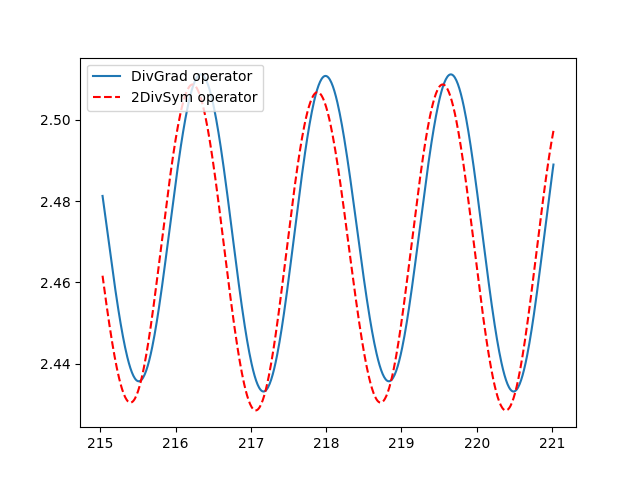
\includegraphics[width=0.5\linewidth]{PressureDifference.png}
	\caption{The pressure difference of both formulations}
	\label{Fig:Pressure}
\end{figure}
\begin{figure}
	\centering
	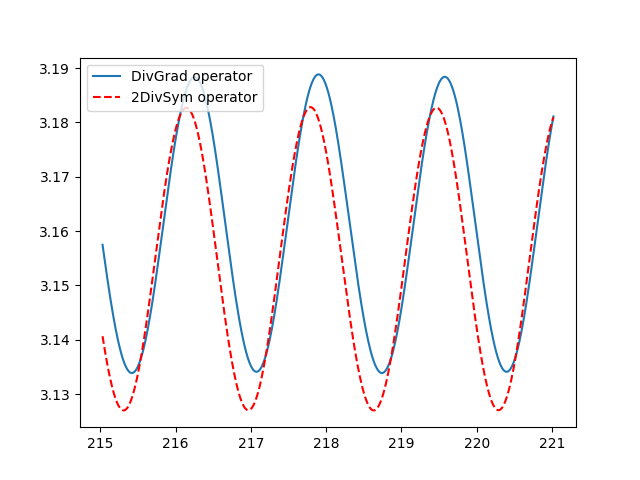
\includegraphics[width=0.5\linewidth]{DragCoefficient.png}
	\caption{The drag coefficient of both formulations}
	\label{Fig:Drag}
\end{figure}
\begin{figure}
	\centering
	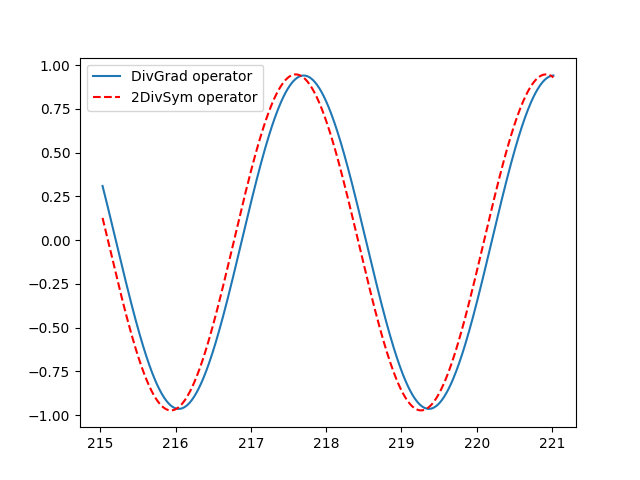
\includegraphics[width=0.5\linewidth]{LiftCoefficient.png}
	\caption{The lift coefficient of both formulations}
	\label{Fig:Lift}
\end{figure}
As you see, the results coincide in a pretty decent manner with those of the benchmark now. According to the Remark 10.1 of the \textsc{Guermond} paper, one may enforce the \cref{Eqn:CylinderForce} if one also replaces the \textsc{Laplace} operator in the diffusion step by $\nabla \cdot \Sym (\nabla \otimes \mathbf{u})$. The thing is, that \textsc{Laplace} operator is applied always to the velocity field $\mathbf{u}$, independent of which projection scheme is used or if the divergence free velocity $\mathbf{v}$ was eliminated or not. Should not the \textsc{Laplace} operator be always replaced by the divergence of the symmetric operator?\\
I did another simulation where modified the weak form pertinent to the divergence of the velocity gradient. As seen in \crefrange{Fig:Pressure}{Fig:Lift}, the values (Labeled 2DivSym) are also inside the benchmark range. But the solution behave weird near the inflow boundary. I uploaded a video with the results of using the \textsc{Laplace} operator named "Laplace.ogv" and another one using the $\nabla \cdot \Sym (\nabla \otimes ())$ operator named "Transpose.ogv". In the  "Transpose.ogv" file you can see the mentioned weird behaviour. This might be due to the time step size, the spatial discretization, or the $\nabla \cdot \Sym (\nabla \otimes ())$ operator. But I wanted to discuss the last option before doing tests.
\subsection{Simulation time}
The DFG benchmark websites proposes to simulate 3.5 seconds, then perform a restart and simulate until 30 seconds. At 25 seconds the flow should have stabilized itself according to them. \\
In our simulation the time is scaled (35, 300 and 250 respectively). After the restart, the simulation appears to reach stationary behaviour way sooner
\begin{figure}
	\centering
	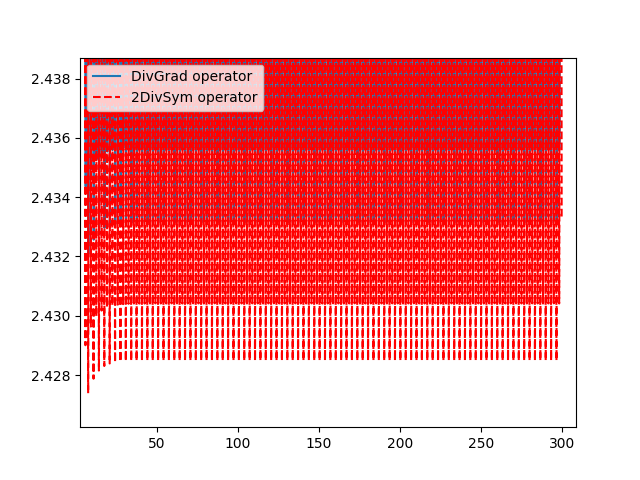
\includegraphics[width=0.5\linewidth]{SimulationTime.png}
	\caption{The lift coefficient of both formulations (Zoomed in)}
	\label{Fig:SimulationTime}
\end{figure}
\end{document}
